\documentclass[a4paper,12pt]{article}

\usepackage[english,brazil]{babel}
\usepackage[utf8]{inputenc}
\usepackage{icomma}
\usepackage{amsmath}
\usepackage{makecell}
\usepackage{graphicx}
\usepackage{fancyhdr}
\usepackage{url}
\renewcommand{\baselinestretch}{1.5}
\usepackage{titling}
\usepackage{geometry}
\usepackage{subfigure}
\geometry{
 a4paper,
 left=35mm,
 right=15mm,
 top=1in,
 bottom=1in,
}
\usepackage{amsmath}
\usepackage{amssymb}
\usepackage{subfigure}
\usepackage{multirow}
\usepackage[table]{xcolor}
\usepackage[backend=bibtex,style=ieee,sorting=none]{biblatex}
\usepackage{algorithm}
\usepackage[noend]{algpseudocode}
\usepackage{pdfpages}
\bibliography{bibliography}

\newcolumntype{C}{>{\centering\arraybackslash}p{1em}}


\newpage

\begin{document}
\selectlanguage{brazil}

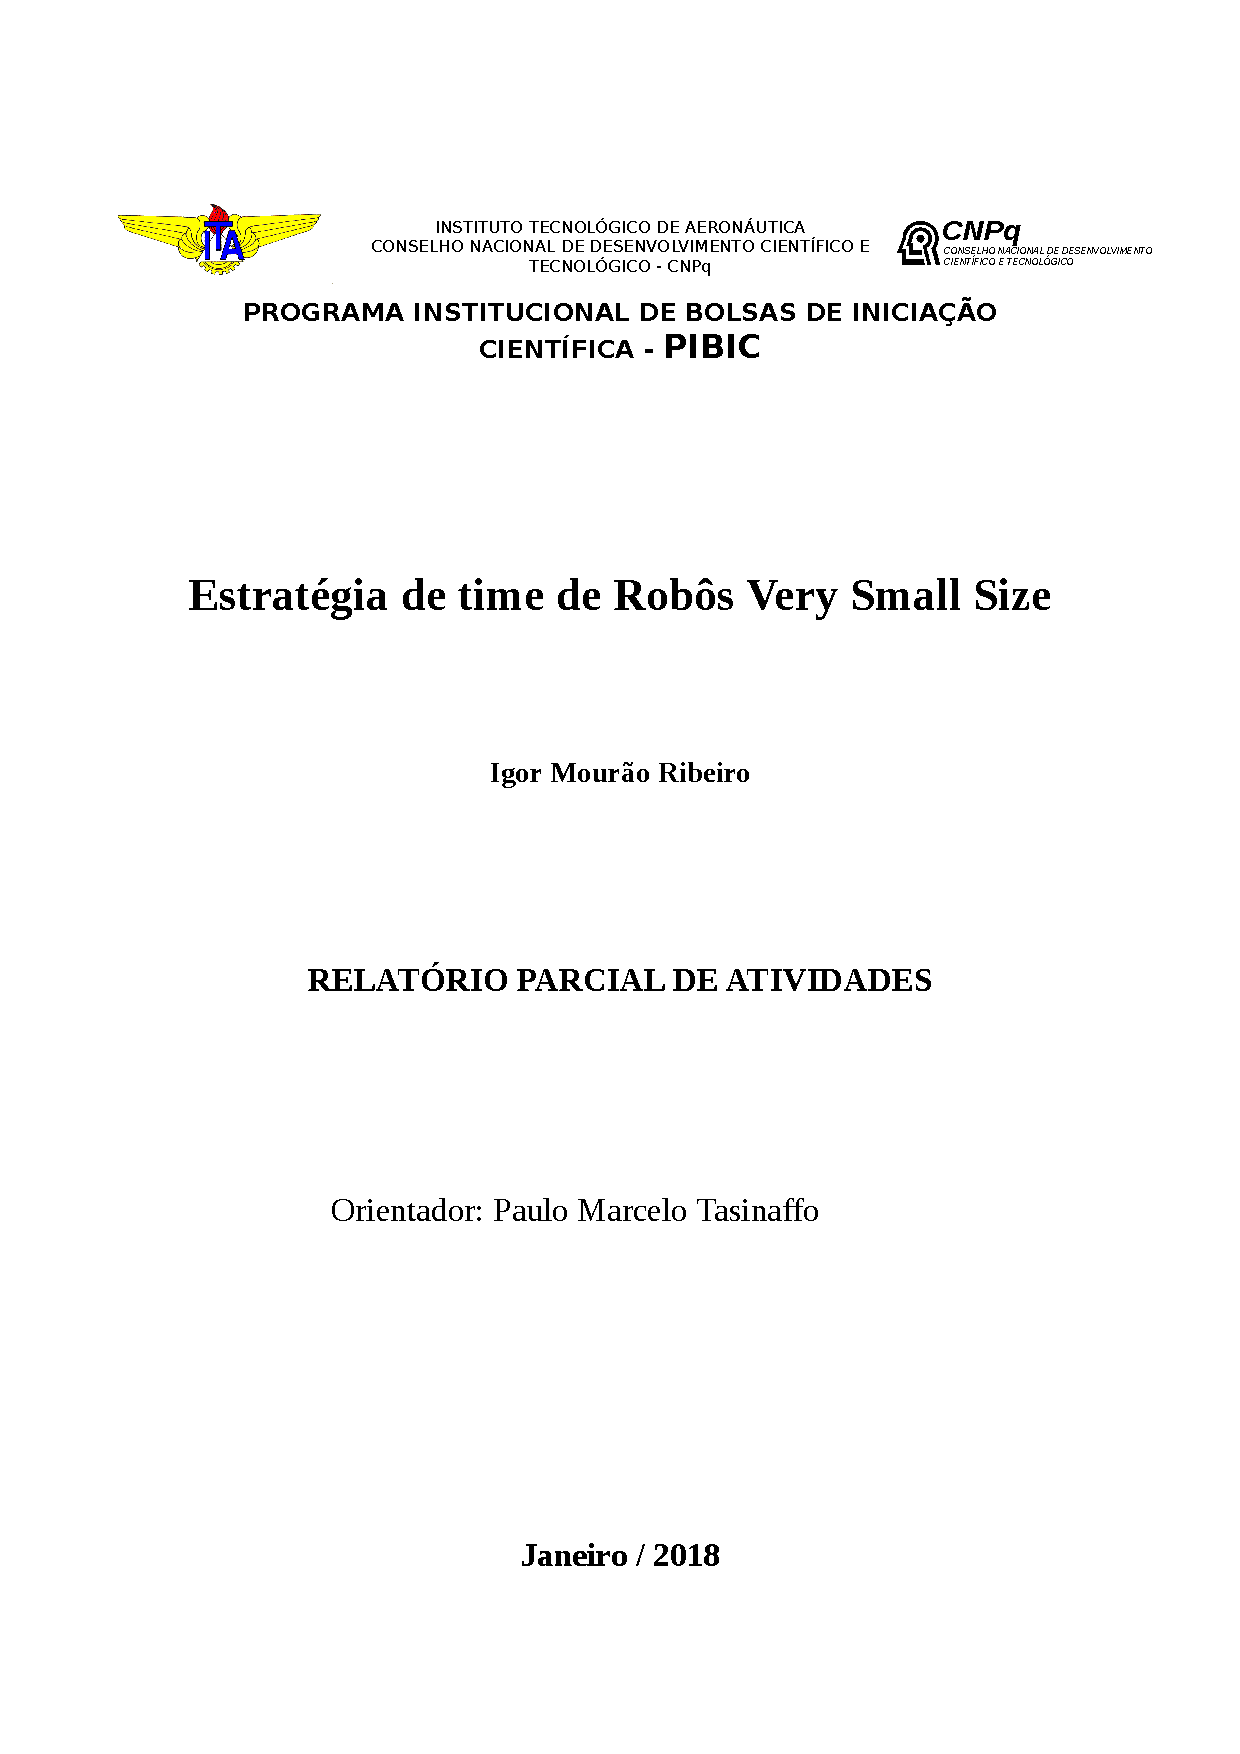
\includepdf[pages={1-},scale=1]{Inicio.pdf}


\tableofcontents

\newpage

\section{Resumo do Plano Inicial}
\label{secao:plano_inicial}

O objetivo deste trabalho é desenvolver e implementar um algoritmo para planejamento de trajetória para um robô diferencial. O contexto é uma partida de futebol segundo a Competição Brasileira de Robótica (CBR), categoria IEEE Very Small Size Soccer. A partir da posição do robô, da bola e dos oponentes no campo, traçar a melhor trajetória para que ele chegue à bola com o ângulo adequado e leve-a ao gol oponente considerando as limitações mecânicas – o robô recebe apenas as velocidades das duas rodas. Visa-se utilizar os algoritmos aqui implementados pela equipe da ITAndroids, que representa o ITA, na competição da Latin America Robotics Competition (LARC)/CBR de 2015 em diante.

Planejamento:
\begin{itemize}

\item 1o Bimestre (ago / set): Estudo da literatura e revisão bibliográfica sobre o tema de planejamento de trajetórias na presença de obstáculos.

\item 2o Bimestre (out / nov): Seleção de métodos a serem implementados para planejamento e codificação da implementação.

\item 3o Bimestre (dez / jan): Simulações computacionais da aplicação dos métodos para cenário simplificado: um robô e obstáculos fixos. Redação do relatório parcial.

\item 4o Bimestre (fev / mar): Simulações computacionais da aplicação dos métodos em cenários realistas de futebol de robôs: múltiplos robôs e obstáculos móveis.

\item 5o Bimestre (abr / mai): Análise dos algoritmos implementados em termos de carga computacional e eficácia.

\item 6o Bimestre (jun / jul): Redação do relatório final. Redação do artigo para o ENCITA.

\end{itemize}

\section{Resumo das Atividades Realizadas}
\label{secao:atividades_realizadas}

Ao longo do primeiro mês, foram realizados estudos e foi decidido que será usado um sistema de controle preditivo para a navegação e controle do robô. A seguir, no segundo mês, foram escolhidos três métodos de planejamento de trajetórias para serem implementados e repassados ao controlador: um baseado em campos potenciais, um em Rapidly-exploring Random Tree (RRT), e um modelando o problema de navegação como um de otimização.

Ao longo do segundo e terceiro bimestres, os algoritmos foram todos implementados utilizando a plataforma MATLAB e foi realizada a simulação para o cenário simplificado (nenhum obstáculo móvel). Foi realizado o ajuste de constantes e os dois primeiros mostraram resultados satisfatórios e condizentes com o que foi previsto. No quarto bimestre, foi realizado o levantamento da carga computacional para ambos os métodos, além de otimizações.

O método de campos potenciais foi implementado em C++ e testado no robô real para uso efetivo na competição, ocorrida entre os dias 28 de outubro e 1 de novembro de 2015. As funções de desvio de obstáculos apresentaram problemas de codificação. O algoritmo, porém, funcionou perfeitamente com estas funções desativadas. A equipe da ITAndroids conquistou o quarto lugar de 30.

O algoritmo de RRT foi implementado em C++ de forma compatível com o robô real e os testes desse código em cenário realista foram feitos com o auxílio do MATLAB. O método de modelar o problema de navegação como de otimização foi testado e reprovado no requisito de tempo e de precisão ainda na simulação com cenário simples.

\section{Descrição do Problema}
\label{secao:enunciado_problema}

No contexto da Robótica, a navegação traz muitos novos desafios. Existe uma diferença muito grande entre ter um robô com um controlador bem implementado e funcional e ter um algoritmo que utilize esse controlador da melhor maneira possível. Isso nos traz a um desafio de nível mais alto: planejar uma trajetória executável pelo controle que permita ao robô executar a tarefa desejada.

Nesse projeto, trabalhou-se com os robôs da competição IEEE Very Small Size: uma competição de futebol de robôs completamente automatizada em que cada robô tem como tamanho máximo um cubo de 7,5 cm de aresta. O campo de futebol possuil 1,5 m de comprimento e 1,3 m de largura. Cada time tem 3 jogadores: um atacante, um defensor e um goleiro. Uma câmera proporciona a visão aérea com as posições de todos os elementos da partida. As regras completas podem ser lidas em \cite{cbr2008}. 

O robô foi projetado com duas rodas laterais e duas esferas livres à frente e atrás para manter o equilíbrio. Essa característica o torna um robô diferencial. Ou seja, temos o controle sobre as velocidades linear e angular.

\begin{figure}
	\label{fig: vss}
	\centering
	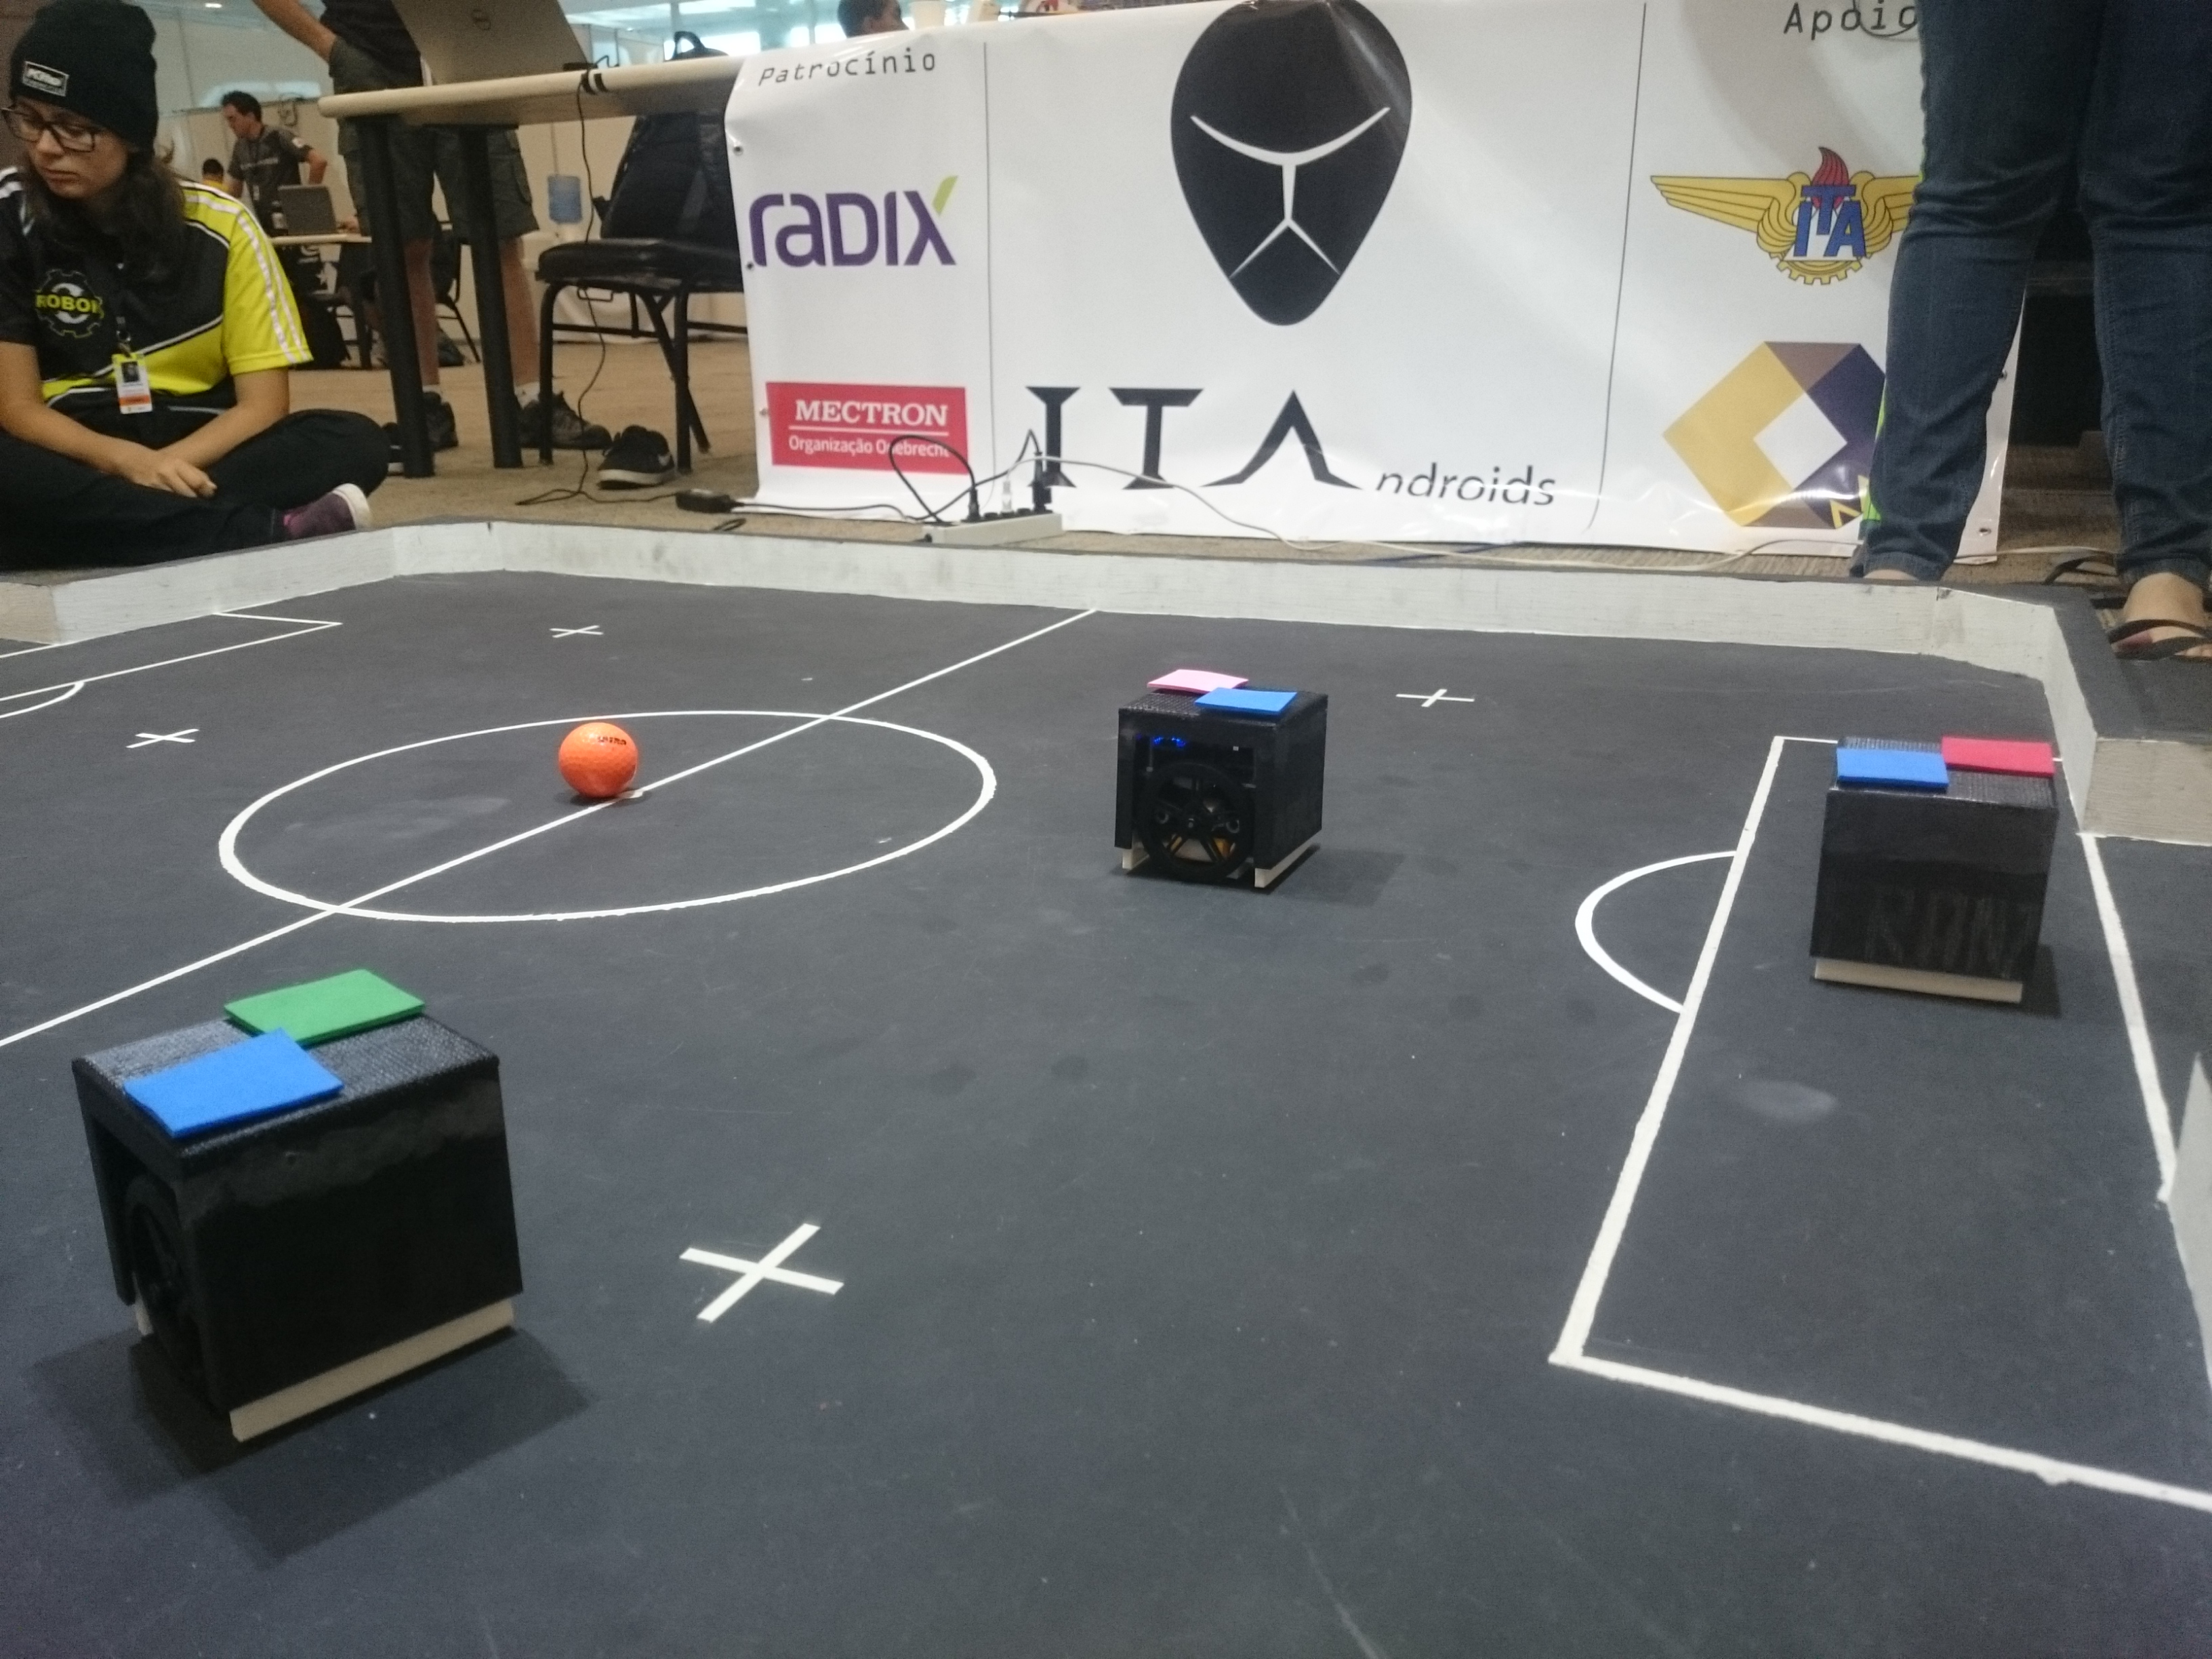
\includegraphics[width=0.5\textwidth]{figures/vss.JPG}
   \caption{A categoria IEEE VSS.}
\end{figure}

Nesse contexto, surgem várias questões a serem resolvidas para se ter um time vencedor. Nesse projeto abordaremos o problema do planejamento de trajetórias: dada a posição inicial do robô, sua velocidade atual, a posição desejada e a velocidade desejada ao se chegar nessa posição, deve-se montar uma trajetória - uma sequência de posições no espaço e de velocidades.

O algoritmo de planejamento de trajetória deve: executar em tempo hábil para o processamento - a frequência de execução do time é de 30 Hz, deixando cerca de 2 ms para o planejamento de trajetórias; levar em consideração todas as restrições de robô diferencial; desviar de possíveis obstáculos (outros jogadores) e não colidir com paredes; retornar uma trajetória ótima de forma a maximizar a eficiência do time; e retornar uma sequência de velocidades aplicável pelo controlador.

%O algoritmo de planejamento de trajetória deve:
%\begin{enumerate}
%\item executar em tempo hábil para o processamento - a frequência de execução do time é de 30 Hz, deixando cerca de 2 ms para o planejamento de trajetórias;
%\item levar em consideração todas as restrições de robô diferencial;
%\item desviar de possíveis obstáculos (outros jogadores) e não colidir com paredes;
%\item retornar uma trajetória ótima de forma a maximizar a eficiência do time; e
%\item retornar uma sequência de velocidades aplicável pelo controlador.
%\end{enumerate}

Para resolver esse problema, foram escolhidos três algoritmos para a modelagem do ambiente e para o cálculo da trajetória: um baseado em campo potenciais e descida gradiente, um baseado em Rapidly-exploring Random Tree (RRT) e um modelando o problema de navegação como um de otimização usando Controle Preditivo e com artifícios de Programação Linear Mista-Inteira (\textit{Mixed-Integer Linear Programming} -- MILP).

\subsection{Campos Potenciais}

Seja $S_{0}$ a posição inicial do jogador e $v_{0}$ sua direção inicial. Seja $S_{f}$ a posição desejada e $v_{f}$ a direção com que se deseja chegar a $S_{f}$. A ideia de campos potenciais consiste em modelar o campo com uma função potencial $P(x,y)$, de forma que, executando o algoritmo de descida de gradiente partindo do ponto inicial, gera-se a sequência de pontos $S'(i)$ segundo a seguinte fórmula recursiva:
\begin{equation}
S'(1) = S_{0} + (h/2)v_{0}
\end{equation}
\begin{equation}
S'(i) = S'(i-1) - h\nabla P, i = 2,...,n
\end{equation}

Para escolher uma função P adequada, foi usada a função potencial elétrico com cargas positivas nos obstáculos. Seja a equação de Poisson:
\begin{equation}
\varepsilon \nabla \cdot E = -\varepsilon \nabla ^2 V=\rho = 0
\end{equation}

Pelo teorema do máximo e mínimo, funções com laplaciano zero não podem ter pontos de mínimo não degenerados no interior de um conjunto em que são analíticas. Isso faz com que o algoritmo convirja para alguma singularidade negativa ou divirja. Assim sendo, basta colocar uma carga negativa no ponto desejado, o que produz uma singularidade negativa naquele ponto.

Como o espaçamento entre os pontos é constante, pode-se obter a sequência de posições $S(i)$ e de direções $v(i)$ da seguinte maneira: A posição por onde passará o robô é o ponto médio entre dois pontos calculados $S'(i)$ e $S'(i-1)$. O módulo de $v(i)$ é unitário e sua direção e sentido coincidem com o vetor $S'(i-1)$ a $S'(i)$. $v(1) = v_{0}$. As equações para $S(i)$ são dadas a seguir:

\begin{equation}
	S(1) = S_{0}
\end{equation}
\begin{equation}
	S(i) = \frac{(S'(i)+S'(i-1))}{2}, i = 2,3,...,n
\end{equation}
\begin{equation}
	S(n+1) = S'(n) + \frac{h}{2} v_{f}
\end{equation}

A partir destas equações, podemos concordar arcos de circunferência entre os pontos $S(i)$ e $S(i+1)$ segundo a figura \ref{fig: concordancia}.

Para configurar os campos de forma a que eles sejam bem condicionados e produzam uma trajetória adequada, são usados também os seguintes artifícios:

\begin{itemize}
\item Dipolo elétrico no alvo alinhado com a direção de chegada desejada. A carga positiva fica à frente e a negativa atrás. Para que o efeito do dipolo seja sentido em todo o campo, sua carga é da ordem de 100 vezes maior que as outras. O padrão das linhas de campo faz com que a trajetória, que as seguem aproximadamente, chegue no ângulo desejado.
\item Existe um limite para o qual o campo repulsivo atua no dipolo da bola. Entre esse limite e o dobro dele, o campo é multiplicado por um fator que decai continuamente para 0. Em pontos distantes, o alvo é puramente atrativo.
\item Cada parede gera um campo normal à parede que decai pela distância da mesma forma que o campo elétrico de uma carga. O cálculo é feito da seguinte maneira: a fim de calcular o campo da parede em um ponto $C$, projeta-se $C$ na parede e considera-se que seja um obstáculo com uma carga positiva menor.
\item Para que se mantenha uma velocidade constante no robô, pode-se definir um raio de curvatura mínimo $R_{min}$. Para impor esta restrição no algoritmo de campos potenciais, pode-se calcular um $\theta_{max}$ de acordo com a figura \ref{fig: concordancia}. A fórmula é dada a seguir:

\begin{equation}
\theta_{max} = arctan(\frac{4hR_{min}^2}{4R_{min}^2 - h^2})
\end{equation}

\item Caso, durante um passo da descida gradiente, o ângulo entre os trechos $S'(i) - S'(i-1)$ e $S'(i+1) - S'(i)$ seja maior que $\theta_{max}$, faz-se o passo com o ângulo $\theta_{max}$ de forma a que $S'(i+1)$ seja o mais próximo possível do que se fosse usado o ângulo do campo.
\end{itemize}

\begin{figure}
	\label{fig: concordancia}
	\centering
	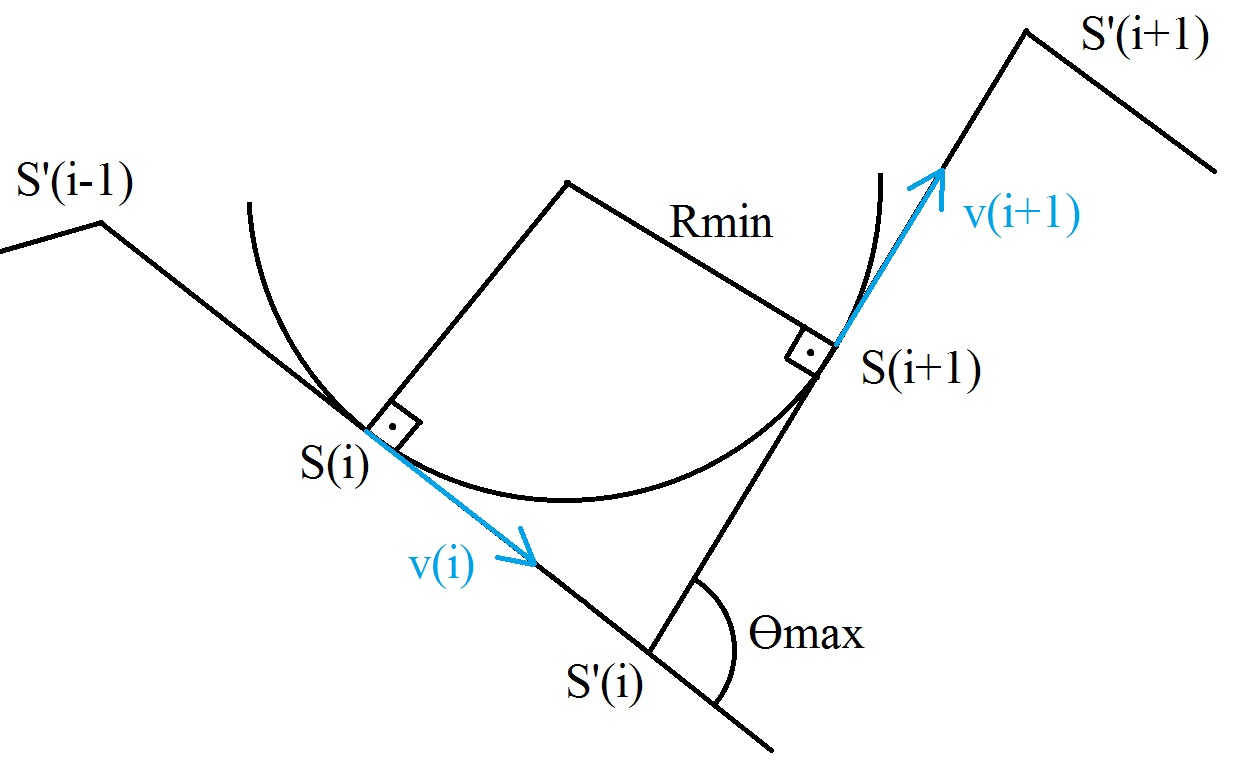
\includegraphics[width=0.5\textwidth]{figures/thetamax.jpg}
   \caption{Circunferência concordada por dois trechos de S' e tangenciando em S}
\end{figure}

\subsection{RRT}

Este algoritmo consiste em expandir árvores em direções aleatórias a partir da posição do robô e do alvo. Durante a expansão, quando dois nós, um de cada árvore, estiverem a uma distância menor que um parâmetro $h$, conecta-se esses dois nós e forma-se um caminho do robô até o alvo. O fator de aleatoriedade garante uma probabilidade admissível de se achar um caminho. Para que sejam respeitadas as restrições do campo e dos obstáculos, basta que os vértices as respeitem. O algoritmo foi estudado segundo a aula \cite{lavalle2011}.

Para minimizar o tempo de expansão, deve-se evitar que duas arestas - os segmentos de reta no espaço que ligam dois vértices vizinhos - se interceptem. Para manter o bom condicionamento e otimizar o cálculo entre duas iterações, devem-se definir probabilidades $G$ de se escolher como novo ponto a raiz da outra árvore e $P$ a de se escolher um ponto da última trajetória calculada. A função $PA$ (Ponto Aleatório) retorna tal ponto. A técnica foi proposta segundo o artigo \cite{james2002}. Para isso, foram implementadas as seguintes funções:

\begin{figure}
	\label{fig: rrt_extend}
	\centering
	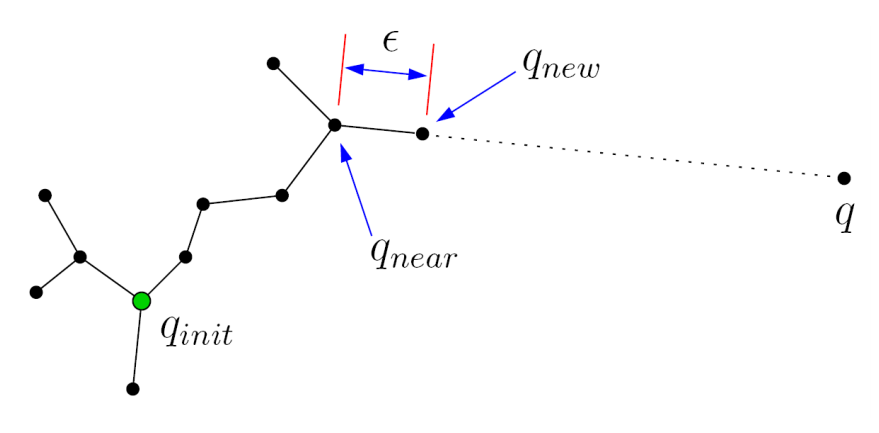
\includegraphics[width=0.5\textwidth]{figures/RRT.png}
   \caption{Exemplo de passo de extensão do RRT. Fonte: LaValle, 2000 e \cite{lavalle2011}}
\end{figure}

\makeatletter
\def\BState{\State\hskip-\ALG@thistlm}
\makeatother

\begin{figure*}[ttt!]

\begin{minipage}[t]{0.5\textwidth}

\begin{algorithm}[H]
\caption{função Estender}\label{euclid}
\begin{algorithmic}[1]
\Procedure{Estender (Árvore $T$, Ponto $q$)}{}
\State $\textit{$q_{near}$} \gets \text{PontoMaisPróximoDe($T$, $q$)}$
\State $\textit{$n$} \gets \text{direção de $q_{near}$ a $q$}$
\BState \emph{loop}:

\If {($q_{near}+n*h$ é válido e $d(q, q_{near}) > d(q, q_{near}+n*h)$}
\State $\textit{Adiciona $q_{near}+n*h$ a $T$}$.
\State $\textit{Liga $q_{near}+n*h$ a $q_{near}$}$.
\State $q_{near} \gets q_{near}+n*h$.
\State \textbf{goto} \emph{loop}.
\State \textbf{close};
\EndIf

\State \textbf{return} \emph{$q_{near}$}.
\EndProcedure
\end{algorithmic}
\end{algorithm}

\end{minipage}
\hfill
\begin{minipage}[t]{0.5\textwidth}

\begin{algorithm}[H]
\caption{função CalcularTrajetória}\label{euclid}
\begin{algorithmic}[1]
\Procedure{CalcularTrajetória ($S_{0}$, $v_{0}$, $S_{f}$, $v_{f}$)}{}
\State $T_{a} \gets S_{0}+(h/2)*v_{0}$
\State $T_{b} \gets S_{f}-(h/2)*v_{f}$
\BState \emph{loop}:

\If {$\textit{($|T_{a}| \leq M$ e $|T_{b}| \leq M$)}$}
\State $P_A \gets \textit{Estender($T_{a}$, PAl)}$.
\State $P_B \gets \textit{Estender($T_{b}$, $P_A$)}$.
\If {$d(P_A, P_B) \leq h$}
\State \textbf{close} \emph{loop}.
\EndIf
\State $\textit{Troca $T_{a}$ e $T_{b}$}$.
\State \textbf{goto} \emph{loop}.
\State \textbf{close};
\EndIf

\State \textbf{return} \emph{Trajetória raiz($T_{a}$)-$P_A$-$P_B$-raiz($T_{b}$)}.
\EndProcedure
\end{algorithmic}
\end{algorithm}

 \end{minipage}

 \hfill

\end{figure*}

É necessário também colocar um limite no número de nós das árvores para que, caso não haja caminho possível, o algoritmo não entre em loop infinito. Para garantir que sejam respeitadas as direções iniciais e finais, adicionaram-se obstáculos ao lado das posições finais e iniciais, de forma que as árvores possam expandir apenas se alinhando entre eles.

Para se otimizar o passo de escolher o ponto $q_{near}$ de uma árvore mais próximo a um ponto $Q$, foi implementada a estrutura de dados Quadtree, que permite a inserção e busca de ponto mais próximo em $O(\log{n})$, enquanto a inserção e busca normais são, respctivamente, $O(1)$ e $O(n)$. Os resultados de ambos os métodos foram comparados.

Um dos problemas identificados é a possibilidade de mal condicionamento do algoritmo: a cada passo, ele pode gerar um caminho distinto. Além do caminho atual ser orientado para ser semelhante ao da iteração anterior, deve-se executar o algoritmo várias vezes e tomar o menor caminho de cada execução. O menor caminho converge para o mínimo possível.

Deve-se, também, suavizar a trajetória. Percorre-se a trajetória inteira calculando os ângulos entre dois trechos. Caso esse ângulo ultrapasse um limite $\theta_{max}$, definido e calculado a partir de $R_{min}$ da mesma forma descrita nos campos potenciais, elimina-se esse ponto da trajetória e liga-se seus pontos adjacentes. No passo de suavização por arcos de circunferência e na ponte entre as duas árvores, pode-se gerar trechos que não têm tamanho $h$. Basta alterar a concordância dos arcos para que eles comecem ou terminem na metade do trecho de menor comprimento. Assim, basta uma pequena alteração nas equações de concordância para que se obtenham as sequências finais $S$ e $v$ e as velocidades linear e angular.

\subsection{Otimização com Mixed Integer-Linear Programming (MILP)}

Modelar um problema qualquer como um problema de otimização significa definir uma função de erro cujo ponto de mínimo que respeita um conjunto de restrições é a solução. A partir disso, pode-se usar algoritmos computacionais para achar esse ponto.

Foi utlizado, para realizar este cálculo, a biblioteca GLPK para MATLAB. A vantagem dela é o trabalho com Programação Linear Mista-Inteira, o que permite adicionar restrições de tipo nos vetores de variáveis: eles podem ser de reais, inteiros ou binários com limites inferior e superior.

Primeiro definimos a função de custo e as restrições como 
\begin{equation}
	\label{eq:custo}
	J(b) = \sum_{i=1}^{\log_2 {N}} b(i)2^{i-1} = n,
\end{equation}
\begin{equation}
	\label{eq:restr}
	Av \leq B \; ou \; \sum_{j=1}^{N_{var}} A_{ij}v(j)  \leqslant B_i
\end{equation}

onde $N$ é o número máximo de passos para a trajetória tomado sempre como potência de $2$ e $N_{ver}$ o número de veriáveis. $b(i)$ é um vetor de variáveis binárias que representa a codificação binária de $n$, o número de passos utilizados. Minimizar $J(b)$ significa percorrer o caminho com o mínimo de passos possíveis.

O pacote GLPK permite adicionar restrições por meio da equação \eqref{eq:restr}, onde $A$ é uma matriz inserida pelo usuário, $v$ é a concatenação de todos os vetores de variáveis (reais, inteiras e binárias) e $B$ é um vetor de constantes também definido pelo usuário. O algoritmo determinará $v$ de forma a que todas as inequações contidas em \eqref{eq:restr} sejam satisfeitas e que $J(b)$ seja minimizado.

Isso significa que podemos adicionar desigualdades sobre uma determinada combinação linear de variáveis. Para preencher as matrizes $A$ e $B$ com os valores que representem todas as retrições do problema, foram feitas duas abordagens.

\subsubsection{Navegação sobre todo o campo}

Nesta abordagem, teremos como variáveis controladas pelo otimizador a parte positiva e negativa das acelerações em $x$ ($x_{p}$ e $x_{n}$, respectivamente) e em $y$ ($y_{p}$ e $y_{n}$, respectivamente). Impõem-se restrições de mínimo zero e máximo $a_{max}$. Sejam $u(i)$ a aceleração no i-ésimo passo, ou seja, $u(i) = (x_{p}(i)-x_{n}(i), y_{p}(i)-y_{n}(i))$, $T$ o tempo de cada passo, $S(1)=S_{0}$ e $v(1)=v_{0}$ as posições iniciais do robô, então as equações para o movimento na i-ésima posição são:

\begin{equation}
	v(i) = v(1) + T\sum_{j=1}^{i-1}u(j)
\end{equation}
\begin{equation}
	S(i) = S(1) + (i-1)Tv(1) + T^2\sum_{j=1}^{i-1}(n-j-\frac{1}{2})u(j)
\end{equation}

Para restringir a velocidade máxima, basta adicionar desigualdades do tipo:

\begin{equation}
	-V_{max} \leq v(i)_x, v(i)_y \leq V_{max}
\end{equation}

Seja $\epsilon$ um erro admissível para a posição final do robô. Para se chegar na posição final desejada com a direção desejada, devemos adicionar restrições sobre a n-ésima posição calculada. Seja $bin(i,j)$ o j-ésimo algarismo de $i$ em sua representação binária. Para implementar dessa maneira, adiciona-se um termo extra $C(i,b)$ definido da seguinte forma:
\begin{equation}
    C(i,b) = \sum_{j=0}^{\log_2{N}} c(i,j)b(j)
\end{equation}
\begin{equation}
    c(i,0) = \sum_{j=1}^{\log_2 {N}} bin(i,j) \qquad
    c(i,j) = \left\{ \begin{array}{r} 1, se\ bin(i,j) = 0 \\ 
    -1, se\ bin(i,j) = 1
    \end{array} \right.
\end{equation}

$C(i,b)$ é uma função que recebe a representação binária de um inteiro por meio do vetor $b$ e um inteiro $i$. Ela retorna 0 caso $b$ represente $i$ em binário e um valor positivo caso contrário. Seja $M$ um número suficientemente grande. Para $i = 1,...,N$, as inequações de restrição, assim, ficam da seguinte forma:

\begin{equation}
	x_{f} - \epsilon - MC(i,b) \leq S(i)_x \leq x_{f} + \epsilon + MC(i,b)
\end{equation}
\begin{equation}
	y_{f} - \epsilon - MC(i,b) \leq S(i)_y \leq y_{f} + \epsilon + MC(i,b)
\end{equation}

Dessa forma, quando o otimizador escolher um valor para $n$ por meio de $b$, essas equações serão relaxadas (reduzidas a $\infty \geq x$) para passos diferentes de $n$ e impostas (último termo eliminado) caso contrário. Da mesma forma, garantimos que a velocidade de chegada seja a desejada por meio das equações:

\begin{equation}
	v_{fx} - \epsilon - MC(i,b) \leq v(i)_x \leq v_{fx} + \epsilon + MC(i,b)
\end{equation}
\begin{equation}
	v_{fy} - \epsilon - MC(i,b) \leq v(i)_y \leq v_{fy} + \epsilon + MC(i,b)
\end{equation}

Para as restrições de campo, basta adicionar as desigualdades:

\begin{equation}
	-X_{max} \leqslant S(i)_{x} \leqslant X_{max}, \qquad -Y_{max} \leqslant S(i)_{y} \leqslant Y_{max}
\end{equation}

Enfim, para representar as restrições de obstáculos, modelou-se cada um como um quadrado de aresta $L$. Adicionaram-se duas variáveis binárias que formam números de 0 a 3 para cada obstáculo. A função $obs(i, j)$, para o i-ésimo passo e para o j-ésimo obstáculo, representa a seguinte codificação:

\begin{itemize}
\item $obs(i, j) = 0$: posição abaixo da linha inferior do obstáculo.
\item $obs(i, j) = 1$: posição à direita da linha direita do obstáculo.
\item $obs(i, j) = 2$: posição acima da linha superior do obstáculo.
\item $obs(i, j) = 3$: posição à esquerda da linha esquerda do obstáculo.
\end{itemize}

Logo, para todo i e j, basta adicionar restrições do tipo:

\begin{equation}
	x_{obs}(j) +  \frac{L}{2} - \epsilon - MC(1,obs(i,j)) \leq S(i)_x \leq x_{obs}(j) - \frac{L}{2} + \epsilon + MC(3,obs(i,j))
\end{equation}
\begin{equation}
	y_{obs}(j) +  \frac{L}{2} - \epsilon - MC(0,obs(i,j)) \leq S(i)_y \leq y_{obs}(j) -  \frac{L}{2} + \epsilon  + MC(2,obs(i,j))
\end{equation}

\subsubsection{Navegação por uma triangulação}

Outro jeito de se utilizar o GLPK é da seguinte maneira: suponha que tenhamos uma sequência de triângulos adjacentes tal que o ponto de saída está no primeiro triângulo e o de chegada, no último. Podemos usar o pacote para achar a trajetória por dentro de um triângulo até o próximo.

Para impôr as restrições de desvio de obstáculos e de parede, usa-se as quinas do campo e as pontas dos obstáculos para computar a triangulação de Delaunay \cite{delaunay34}. Assim, podemos obter um grafo de triângulos por onde poderemos estimar o melhor caminho. Basta utilizar o algoritmo de Dijkstra \cite{dijkstra59} sobre o grafo de Voronoi \cite{voronoi08} ou no dos centróides para estimar o melhor caminho proibindo a passagem por triângulos no interior de obstáculos.

%\begin{figure}
% 	\begin{minipage}[t]{.48\textwidth}
%		\label{fig:delaunay}
%		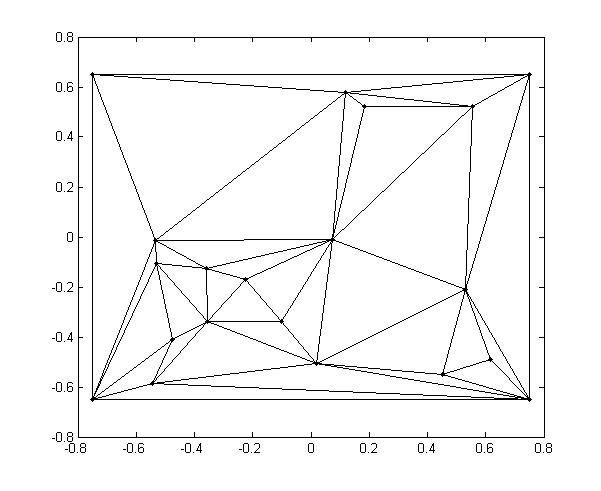
\includegraphics[width=1\textwidth]{figures/delaunay.jpg}
% 		\caption{Triangulação de Delaunay com as quinas do campo e com pontos aleatórios.}
%	\end{minipage}
%   \hfill
%	\begin{minipage}[t]{.48\textwidth}
%		\label{fig: MILP}
%		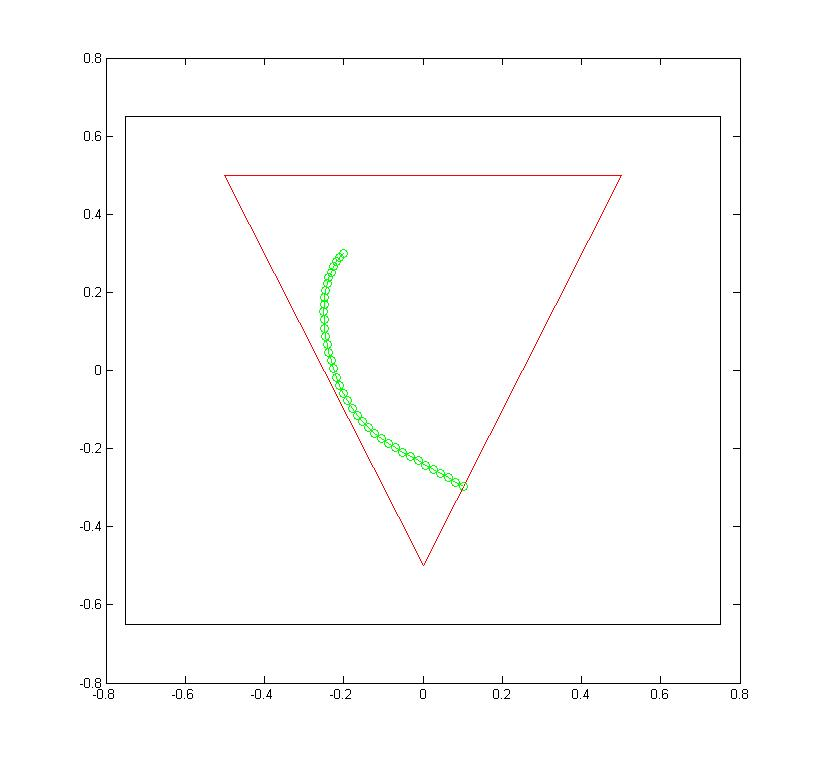
\includegraphics[width=1\textwidth]{figures/MILP.jpg}
%		\caption{Algoritmo de otimização para sair de um triângulo por um lado específico. Neste exemplo, o inferior direito.}
%	\end{minipage}	
%\end{figure}

%\begin{figure}
%  \begin{minipage}[t]{.48\textwidth}
%      \label{fig:voronoi}
%		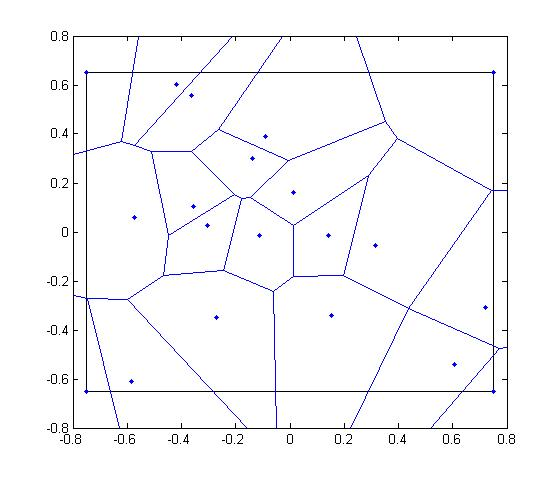
\includegraphics[width=1\textwidth]{figures/voronoi.jpg}
%   		\caption{Grafo de Voronoi. Os pontos representam os obstáculos. As arestas, mediatrizes de dois obstáculos, possíveis caminhos.}
%    \end{minipage}
%    \hfill
%	\begin{minipage}[t]{.48\textwidth}
%    	\label{fig:centroides}
%		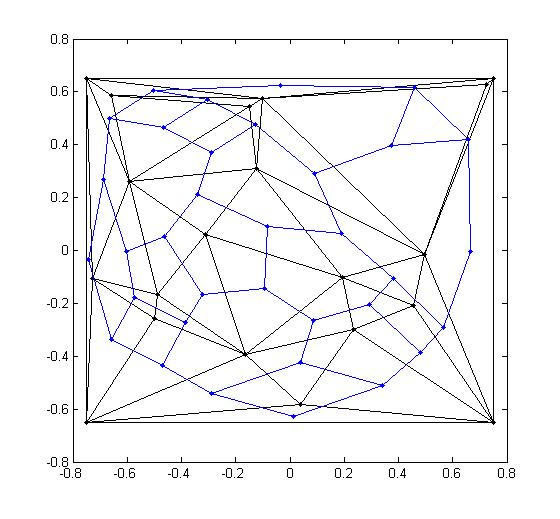
\includegraphics[width=1\textwidth]{figures/centros.jpg}
%  		\caption{Em preto, a triangulação de Delaunay. Em azul, o grafo dos centróides.}
%    \end{minipage}	
%\end{figure}

Modelar o problema desta forma reduz a probabilidade de ele achar a trajetória ótima, mas reduz o tempo de processamento pois não são levados em consideração obstáculos pelo otimizador, diminuindo tanto o número de variáveis binárias quanto de restrições.

Sejam $P1$ e $P2$ os pontos do triângulo do lado por onde o robô quer sair. Seja $P3$ o terceiro ponto. Seja $<,>$ o produto escalar de dois vetores e $\times$ o produto vetorial. A equação \ref{eq: del1} impõe que no n-ésimo passo o robô está do outro lado da reta que caracteriza o lado em comum entre o triângulo atual e o próximo. As equações \ref{eq: del_par1} e \ref{eq: del_par2} impõem que o robô deve estar entre outros dois lados do triângulo em todos os passos.

\begin{tabular}{p{15cm} p{7cm}}
    \vspace{0pt} 
    \label{fig: milp}
	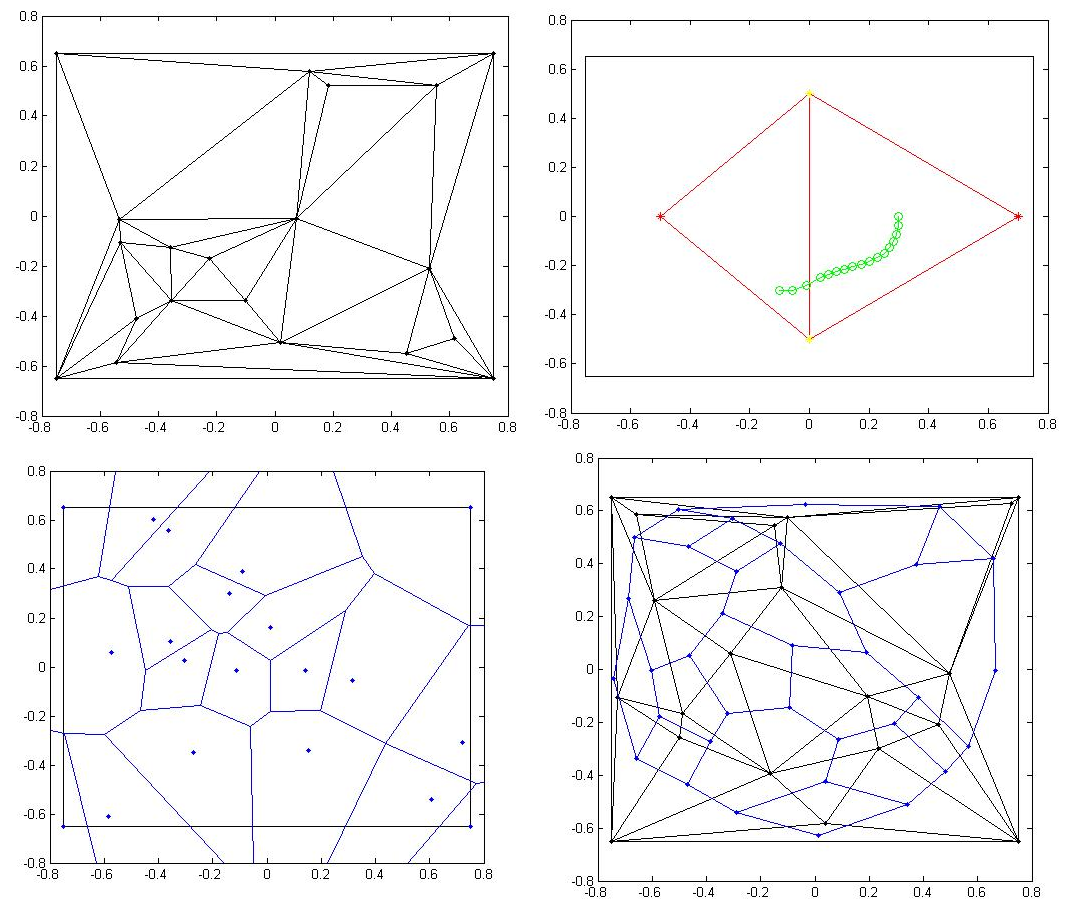
\includegraphics[width=1\textwidth]{figures/allmilp.png}
    \vspace{0pt}\\
    Da esquerda pra direita, de cima pra baixo: triangulação de Delaunay com as quinas do campo e com pontos aleatórios; algoritmo de otimização para sair de um triângulo pelo lado esquerdo; grafo de Voronoi, os pontos representam os obstáculos, as arestas, mediatrizes de dois obstáculos; em preto, a triangulação de Delaunay, em azul, o grafo dos centróides. \\
\end{tabular}

\begin{equation}
\label{eq: del1}
<(S(i)-P1)\times(P2-P1),(P3-P1)\times(P2-P1)>\ \leq \epsilon + MC(i,b)
\end{equation}

\begin{equation}
\label{eq: del_par1}
<(S(i)-P1)\times(P2-P1),(P3-P1)\times(P2-P1)>\ \geq -\epsilon
\end{equation}

\begin{equation}
\label{eq: del_par2}
<(S(i)-P2)\times(P3-P2),(P1-P2)\times(P3-P2)>\ \geq -\epsilon
\end{equation}

\section{Resultados Obtidos}
	\label{secao: resultados_obtidos}
    
No início do trabalho, foi dedicado um mês para estudo de controle preditivo pelo livro \cite{maciejowski2002}, sendo adquirida uma base de conhecimento para nortear como deve ser a resposta do planejador de trajetórias. Não houve, a princípio, dificuldades na escolha dos métodos a serem utilizados. Os três algoritmos apresentados neste projeto foram escolhidos pelos seguintes critérios:

\begin{enumerate}
\item Campos potenciais já é largamente utilizado por equipes da competição IEEE Very Small Size. Em 2014, a ITAndroids tentou sua implementação, porém fracassou. O método foi assim escolhido por ser onipresente na competição e simples para a resolução deste problema.
\item RRT possui uma ampla gama de aplicações acadêmicas em robótica, sendo um método famoso. Em contraste com o anterior, ele é mais complexo e pode resolver o problema para casos mais genéricos: navegação por labirintos e por caminhos estreitos.
\item Otimização por MILP é um algoritmo que, em contraste com os anteriores, é menos empregado em estudos de robótica. Este método pode levar a resultados melhores que os anteriores, além de ser largamente explorado em diversos trabalhos de pesquisa recentes.
\end{enumerate}

Nos meses seguintes, até outubro, com o material passado pelo orientador, nas referências \cite{bellingham2002} e \cite{rubens2015}, foi estudado o método de otimização por MILP para navegação completa pelo mapa. A implementação foi feita em MATLAB, porém seu tempo de execução se mostrou muito longo e o método foi temporariamente descartado. Era necessária uma reformulação do algoritmo para simplificá-lo e torná-lo rápido o bastante.

Na primeira semana de outubro, foi implementado o método de campos potenciais em MATLAB e logo em seguida em C++. A fonte para os estudos foi o artigo \cite{khatib1986}. Foi realizado o teste para o ajuste de parâmetros e para a adaptação de casos especiais.

Nas duas semanas seguintes, prosseguiu-se para o estudo pelas fontes \cite{lavalle2011}, \cite{rubens2009} e \cite{howiechoset} e implementação do método RRT. As implementações em MATLAB e em C++ ficariam prontas ao final de outubro, sendo realizados os testes em cenário simplificado de forma que se pudesse ajustar as constantes e avaliar se o algoritmo seria aplicável ao robô real.

Nessa época, aproximava-se a competição da CBR 2015, sendo interrompida a série de testes do RRT. Foi escolhido o método de campos potenciais para ser utilizado pela ITAndroids. Na última semana de outubro e na primeira de novembro, ele foi testado no robô real. O ITA ganhou quarto lugar na categoria. Apesar do sucesso, foram encontrados vários erros durante os testes e algumas constantes tiveram de ser alteradas para a aplicação no evento. Após a competição, os testes do RRT em cenário simplificado foram concluídos ao longo do mês de novembro.

Durante o período de recesso (dezembro de 2015 a fevereiro de 2016), o método de otimização MILP foi reformulado com a divisão do campo na triangulação de Delaunay. Foi implementado em MATLAB, e nos dois meses seguintes (março e abril de 2016), foram realizados diversos testes em caso simplificado com o algoritmo afim de fazê-lo cumprir com os requisitos do problema. No entanto, os resultados não foram satisfatórios e, desta vez, o método foi definitivamente descartado.

No restante do tempo até a redação do relatório no mês de julho, foram realizadas simulações em cenários realistas para os dois primeiros métodos, sendo medidos os tempos e averiguando se os resultados se enquadram nos requisitos. Mais otimizações foram feitas para o RRT.

A seguir serão apresentados os resultados técnicos dos métodos de campos potenciais e de RRT para o seguinte cenário, com as simulações executadas em um computador com processador Intel Core i7 com \textit{clock} de $2,4 \, GHz$:

\begin{itemize}
\item Posição e direção iniciais, respectivamente: $(0;-0,6)$ e $\frac{1}{\sqrt[]{2}}(-1;1)$
\item Posição e direção finais, respectivamente: $(0;0,6)$ e $\frac{1}{\sqrt[]{2}}(-1;1)$
\item Obstáculos na posições: $(-0,3;0,3)$, $(-0,5;0)$, $(0,1;0)$ e $(0,5;-0,3)$
\end{itemize}
   
\subsection{Campos potenciais}

\begin{figure}
\subfigure[Campos potenciais em MATLAB, trajetória não suavizada.]{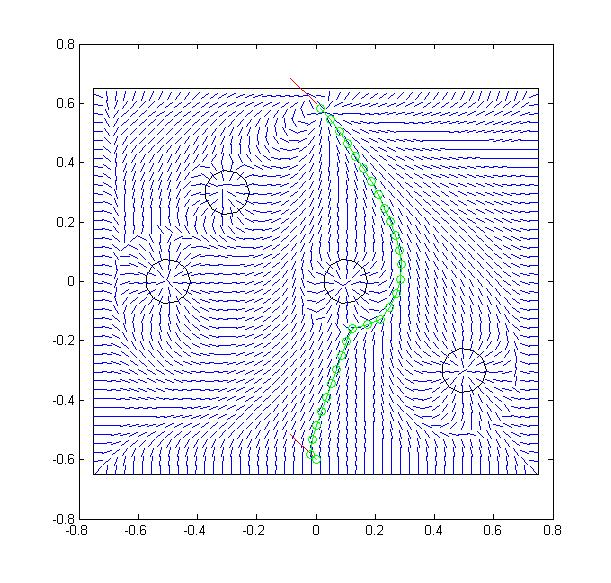
\includegraphics[width=0.47\textwidth]{figures/campospotML.jpg} \label{fig:sub:campospotML}}
\subfigure[Campos potenciais em C++, trajetória suavizada.]{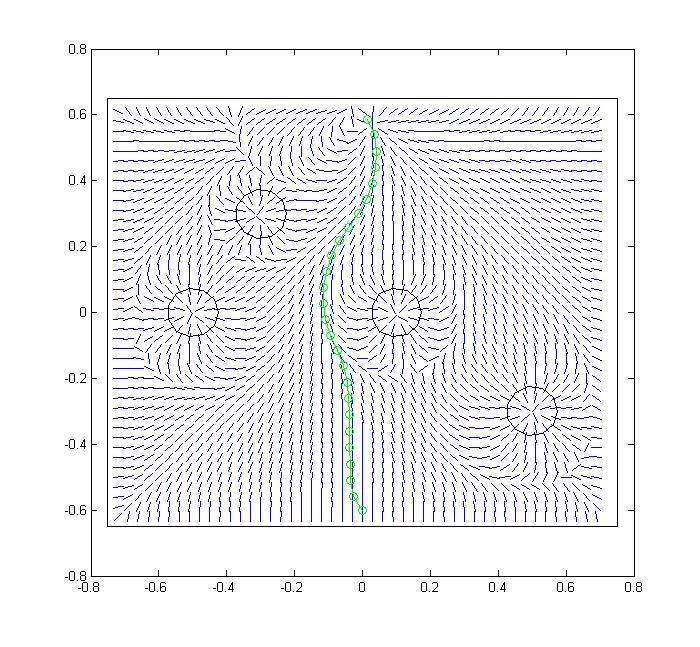
\includegraphics[width=0.47\textwidth]{figures/campospotC++.jpg} \label{fig:sub:campospotC++}}
\caption{Resultados com campos potenciais.}
\end{figure}
    
O algoritmo de campos potenciais foi testado primeiramente na plataforma MATLAB (Fig. \ref{fig:sub:campospotML}) para a configuração das linhas de campo. Em seguida houve o teste em C++ (Fig. \ref{fig:sub:campospotC++}). No primeiro, não foi utilizado o artifício de fazer o campo repulsivo do alvo decair para zero a partir de um limite. Foi observado que não há necessidade de se ter e efeito do dipolo elétrico em todo o espaço, pois o código em C++ gerou, neste teste e em outros, uma trajetória mais suave para o robô.

O tempo de execução foi excelente, sendo de apenas 0,0043 segundos em MATLAB. Em C++ a medição foi de 0,00098 segundos. Isso dá uma boa margem para o requisito de tempo de 2 ms para o planejador de trajetórias, o que o torna um candidato qualificado no quesito tempo.
    
\subsection{RRT}

O método foi testado em MATLAB (Fig. \ref{fig:rrtML}) e em C++ (Fig. \ref{fig:rrtC++}). No primeiro não foi implementada a suavização da trajetória. No segundo, sim.

\begin{figure}
\subfigure[RRT em MATLAB, trajetória não suavizada.]{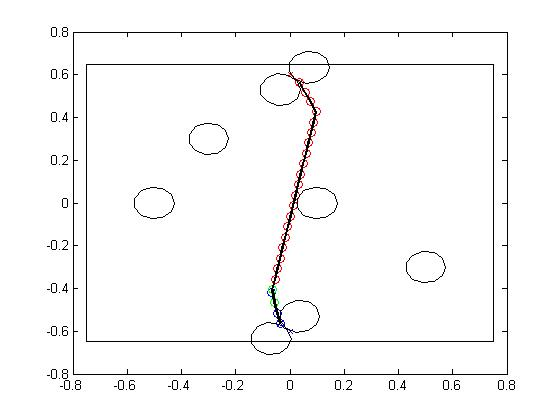
\includegraphics[width=0.47\textwidth]{figures/rrtML.jpg} \label{fig:rrtML}}
\subfigure[RRT em C++, trajetória suavizada.]{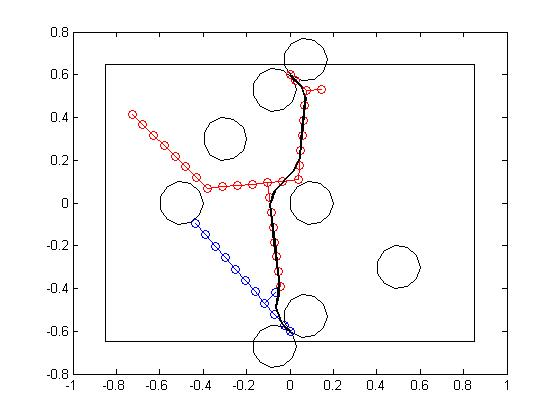
\includegraphics[width=0.47\textwidth]{figures/rrtC++.jpg} \label{fig:rrtC++}}
\caption{Resultados com RRT.}
\end{figure}

Sobre usar ou não usar a Quadtree, o parâmetro $h$ usado foi de $7$ $cm$, fazendo com que a média $n$ de nós das árvores seja da ordem de $50$. A diferença entre o tempo $O(\log{n})$ e $O(n)$ para a inserção, considerando que com o método simples não há alocação de memória e tampouco constantes altas, é pequena. A inserção $O(\log{n})$ com constantes é mais lenta que $O(1)$. O tempo com a Quadtree é aproximadamente o dobro em todos os testes realizados, sendo a estrutura, portanto, descartada.

Nesse caso, devido à característica aleatória do algoritmo, para evitar a variabilidade alta entre duas execuções consecutivas, buscando realmente se aproximar do ótimo, a trajetória é tomada como a melhor (menor comprimento) de um certo número de iterações do mesmo algoritmo. Para fazer a escolha do número de iterações para o algoritmo convergir para a solução ótima, da probabilidade $P$ e da $G$, foram realizados testes de forma a se obter as três tabelas de tempo, em milisegundos, nas tabelas da seção \ref{tab:Tempos_RRT_1}, respectivamente. Cada tempo é a média de $5000$ testes. Deve-se ter $P + G \leq 0,9$, pois deve haver pelo menos $0,1$ de probabilidade de se escolher um ponto aleatório no mapa.

\begin{table}[H]
\caption{Tempos de computação com 5 iterações - média de $5000$ ensaios.}
\centering{
  \begin{tabular}{|c|cccccccc|}
    \hline
    
	$G \backslash P$ & 0.0 & 0.1 & 0.2 & 0.3 & 0.4 & 0.5 & 0.6 & 0.7 \\ \hline
    0.0 & 0,723 & 0,610 & 0,586 & 0,578 & 0,601 & 0,621 & 0,672 & 0,760 \\
    0.1 & 0,804 & 0,621 & 0,599 & 0,608 & 0,642 & 0,683 & 0,761 & 0,939 \\
    0.2 & 0,878 & 0,641 & 0,633 & 0,647 & 0,697 & 0,786 & 0,986 & 1,488 \\
    0.3 & 0,846 & 0,676 & 0,681 & 0,709 & 0,817 & 1,006 & 1,565 & - \\
    0.4 & 1,046 & 0,758 & 0,788 & 0,854 & 1,030 & 1,697 & - & - \\
    0.5 & 1,059 & 0,809 & 0,866 & 1,041 & 1,624 & - & - & - \\
    
	\hline
  \end{tabular}
}
\label{tab:Tempos_RRT_1}
\end{table}

\begin{table}[H]
\caption{Tempos de computação com 10 iterações - média de $5000$ ensaios.}
\centering{
  \begin{tabular}{|c|cccccccc|}
    \hline
    
	$G \backslash P$ & 0.0 & 0.1 & 0.2 & 0.3 & 0.4 & 0.5 & 0.6 & 0.7 \\ \hline
    0.0 & 1,605 & 1,128 & 1,098 & 1,106 & 1,144 & 1,207 & 1,329 & 1,526 \\
    0.1 & 1,530 & 1,179 & 1,155 & 1,174 & 1,243 & 1,380 & 1,575 & 1,969 \\
    0.2 & 1,740 & 1,206 & 1,235 & 1,283 & 1,389 & 1,553 & 1,935 & 3,049 \\
    0.3 & 1,784 & 1,278 & 1,300 & 1,443 & 1,626 & 1,977 & 3,124 & - \\
    0.4 & 2,612 & 1,404 & 1,455 & 1,644 & 2,042 & 3,228 & - & - \\
    0.5 & 2,194 & 1,555 & 1,704 & 2,097 & 3,228 & - & - & - \\
    
	\hline
  \end{tabular}
}
\label{tab:Tempos_RRT_2}
\end{table}

\begin{table}[H]
\caption{Tempos de computação com 25 iterações - média de $5000$ ensaios.}
\centering{
  \begin{tabular}{|c|cccccccc|}
    \hline
	$G \backslash P$ & 0.0 & 0.1 & 0.2 & 0.3 & 0.4 & 0.5 & 0.6 & 0.7 \\ \hline
    0.0 & 3,346 & 2,791 & 2,657 & 2,780 & 2,889 & 2,984 & 3,264 & 3,705 \\
    0.1 & 3,858 & 2,795 & 2,858 & 2,881 & 3,025 & 3,273 & 3,755 & 4,612 \\
    0.2 & 4,100 & 2,887 & 2,913 & 3,077 & 3,332 & 3,823 & 4,749 & 7,698 \\
    0.3 & 4,735 & 3,237 & 3,316 & 3,581 & 4,085 & 5,062 & 8,006 & - \\
    0.4 & 4,788 & 3,552 & 3,730 & 4,210 & 5,231 & 8,177 & - & - \\
    0.5 & 5,405 & 3,985 & 4,400 & 5,395 & 8,326 & - & - & - \\
    
	\hline
  \end{tabular}
  }
\label{tab:Tempos_RRT_3}
\end{table}

A partir dos resultados das tabelas acima, foi decidido usar-se o valor de 0,1 para $G$ e 0,2 para $P$. Em média, o tempo com esses valores é 30\% menor em relação ao algoritmo sem essa heurística (P = G = 0).

Na figura acima, pode-se observar a variança nos caminhos. De esquerda para direita, cima pra baixo: 5, 10, 25 e 100 iterações. Um número menor de iterações é mais rápido, porém existe uma probabilidade maior de se encontrar uma trajetória não ótima e distante da anterior. Diante disso, foi escolhido o número máximo de iterações que respeita o limite de tempo de 2 ms com alguma folga: 15 iterações, que fazem uma média de 1,7 ms.

\subsection{Otimização com MILP}
\subsubsection{Navegação sobre todo o campo}

O método de otimização aplicado sobre todo o campo se mostrou muito lento. O GLPK testa todas as possibilidades de combinações para as variáveis binárias, o que representa uma complexidade de $O(2^n)$. Nessa forma, para cada obstáculo e para cada passo, existem duas variáveis binárias. Por exemplo, para um vetor $b$ com 5 variáveis, existem 32 passos possíveis. Para 5 obstáculos (situação real), existem 10 variáveis binárias. O total de variáveis é de $5 + 32*10 = 325$, o que torna o algoritmo inaplicável para a complexidade dada. O método foi descartado na fase de testes em cenário simples.

\begin{tabular}{p{5cm} p{7cm}}
    \vspace{0pt} 
    \label{fig: rrtsim}
	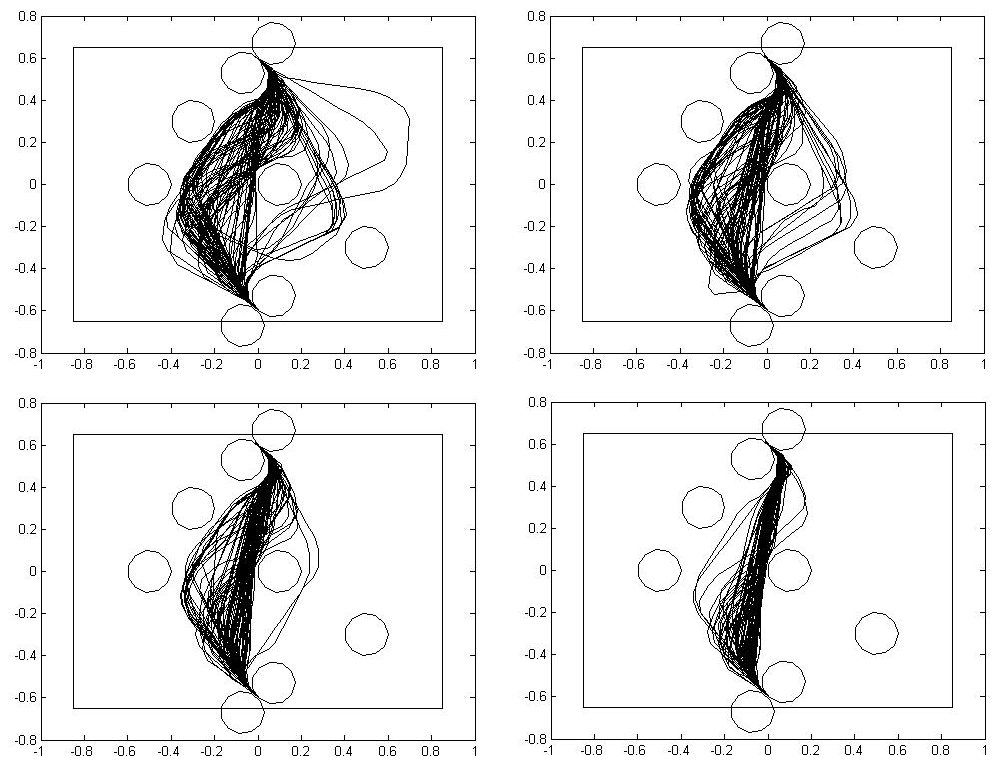
\includegraphics[width=1\textwidth]{figures/allsim.png}
    \vspace{0pt}\\
\end{tabular}

%\begin{figure}
%    \label{fig: rrtsim}
%	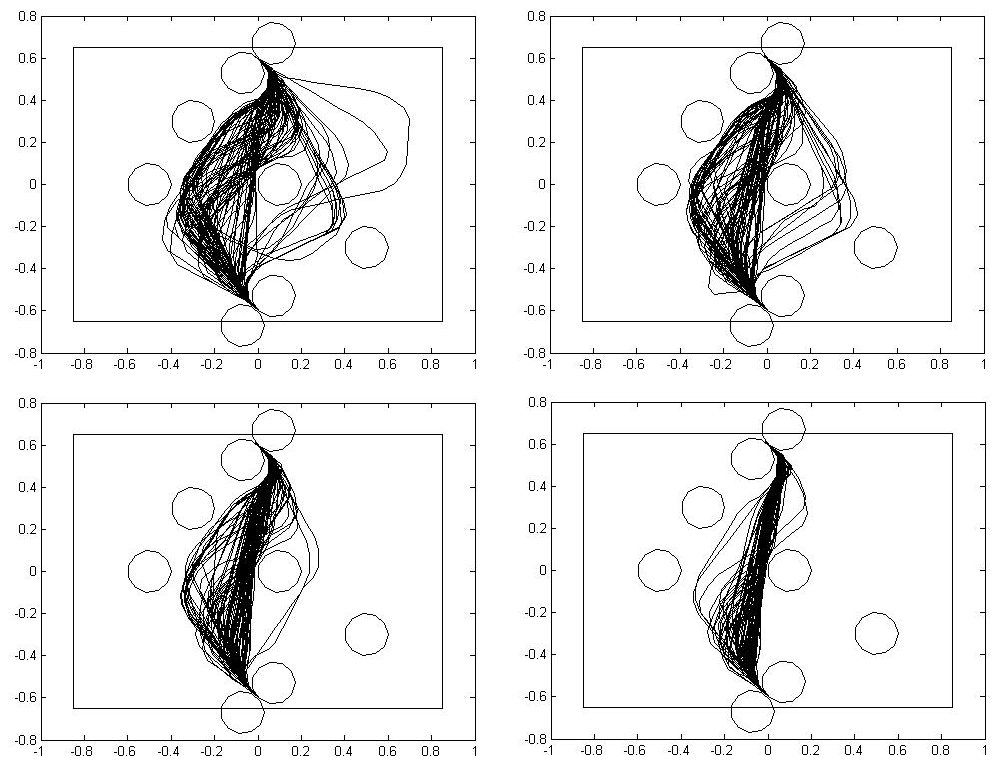
\includegraphics[width=1\textwidth]{figures/allsim.png}
%   	\caption{De esquerda para direita, cima pra baixo: 5, 10, 25 e 100 iterações.}
%\end{figure}

% Na figura acima, pode-se observar a variança nos caminhos. De esquerda para direita, cima pra baixo: 5, 10, 25 e 100 iterações. Um número menor de iterações é mais rápido, porém existe uma probabilidade maior de se encontrar uma trajetória não ótima e distante da anterior. Diante disso, foi escolhido o número máximo de iterações que respeita o limite de tempo de 2 ms com alguma folga: 15 iterações, que fazem uma média de 1,7 ms.

% \subsection{Otimização com MILP}
% \subsubsection{Navegação sobre todo o campo}

% O método de otimização aplicado sobre todo o campo se mostrou muito lento. O GLPK testa todas as possibilidades de combinações para as variáveis binárias, o que representa uma complexidade de $O(2^n)$. Nessa forma, para cada obstáculo e para cada passo, existem duas variáveis binárias. Por exemplo, para um vetor $b$ com 5 variáveis, existem 32 passos possíveis. Para 5 obstáculos (situação real), existem 10 variáveis binárias. O total de variáveis é de $5 + 32*10 = 325$, o que torna o algoritmo inaplicável para a complexidade dada. O método foi descartado na fase de testes em cenário simples.

\subsubsection{Navegação por uma triangulação}

O segundo método, por outro lado, permite o trabalho do GLPK sem levar os obstáculos em consideração, pois ao respeitar o limite dos triângulos, respeita-se ao mesmo tempo a restrição dos obstáculos. Tendo apenas 5 variáveis binárias, a complexidade $O(2^n)$ é admissível. No entando, ao se dividir o problema em triângulos e montar um algoritmo que resolve a transição por um triângulo, o algoritmo passou a não respeitar possíveis restrições do próximo triângulo enquanto soluciona o atual.

Por exemplo, foi usado para testes um gerador de situações aleatórias, que posiciona 5 obstáculos (três adversários e dois aliados) no campo. O otimizador leva o robô ao próximo triângulo com sucesso, entrentanto ele chega com uma posição e direção desfavoráveis para a solução do próximo. Em mais da metade dos testes aleatórios, o otimizador GLPK acusou erro de equação sem solução para algum trecho.

Tentar expandir as restrições do triângulo seguinte para o atual acabou por exigir uma quantidade maior de equações de restrição, o que desacelerou o algoritmo e acabou por não conseguir resolver inteiramente o problema. Diante dessa situação, este método também foi descartado ainda na fase de testes em cenário simples.

\section{Conclusões}

O projeto de Iniciação Científica apresentou bons resultados, especialmete quanto à vitória da equipe do ITA até as semifinais da CBR 2015, rendendo o quarto lugar à equipe. 

Do ponto de vista técnico, o uso do algoritmo já consagrado de planejamento por campos potenciais se mostrou factível em tempo real e adequado para o desvio de obstáculos. Contudo, classes mais gerais de problemas podem ser resolvidos com RRT e MILP, visto que estes podem englobar modelos do robô no planejamento, levando em conta suas limitações ao calcular a trajetória. Por esse motivo, visto as dificuldades com o método de otimização, o RRT foi escolhido para prosseguir com os testes e com a otimização de parâmetros a fim de se montar uma classe de planejamento de trajetórias funcional para a equipe da ITAndroids.

\section{Agradecimentos}

\begin{itemize}
\item Ao CNPq, pelo apoio financeiro e motivacional.
\item À ITAndroids, equipe que representa o ITA na competição da LARC/CBR, pela ideia do projeto, pela disponibilidade do robô real para implementação e oportunidade de aplicação dos métodos estudados.
\item Ao professor Marcos Máximo da Divisão da Ciência da Computação do ITA, pelo apoio nos estudos e no desenvolvimento do projeto.

\end{itemize}

\section{Bibliografia}


\printbibliography[heading=none]

\end{document}